\documentclass[11pt,a4paper]{article}
\usepackage[utf8]{inputenc}
\usepackage[T1]{fontenc}
\usepackage{amsmath,amssymb}
\usepackage{graphicx}
\usepackage{xcolor}
\usepackage{hyperref}
\usepackage{geometry}
\usepackage{tikz}
\usepackage{enumitem}
\usepackage{float}
\usepackage{caption}
\usepackage{booktabs}
\usepackage{fancyhdr}

\geometry{margin=2.0cm,columnsep=0.7cm}
\usetikzlibrary{arrows.meta,positioning,fit,backgrounds}
\hypersetup{colorlinks=true,linkcolor=blue,urlcolor=blue,citecolor=blue}
\definecolor{primary}{RGB}{41,128,185}
\definecolor{success}{RGB}{39,174,96}
\definecolor{accent}{RGB}{211,84,0}
\definecolor{darkgray}{RGB}{44,62,80}
\definecolor{lightgray}{RGB}{245,247,250}

\title{\textbf{Weekly Report}\\[4pt]\large CARLA Fleet Control and Ground-Station Integration}
\author{Qi LI}
\date{July 24, 2026}

\begin{document}
\setcounter{tocdepth}{1}
\twocolumn[
\maketitle
\tableofcontents
\vspace{.3em}
]
\small
\section{Work summary}
This week I completed:
\begin{itemize}[leftmargin=*]
    \item Completed the versioned TCP ground-station bridge, server, command-line interface, and read-only terminal dashboard. And a three-vehicle CARLA fleet scenario is presented here with one leader, two followers, predecessor V2V exchange, and recorded spacing, speed, steering, and fleet-health diagnostics.
    \item Kept the current result focused on platform integration. The observer theory and the SDCS small-map path-following result are deferred to the next weekly report.
\end{itemize}

\section{Fleet control}
\subsection{Fleet composition and runtime flow}
The CARLA experiment contains three vehicles: one leader and two followers. Figure~\ref{fig:fleet-architecture} shows the repeated local structure and data flow. Each vehicle keeps its own local estimate and actuator path; only typed V2V predecessor-state messages are exchanged between vehicles.

\begin{figure*}[t]
\centering
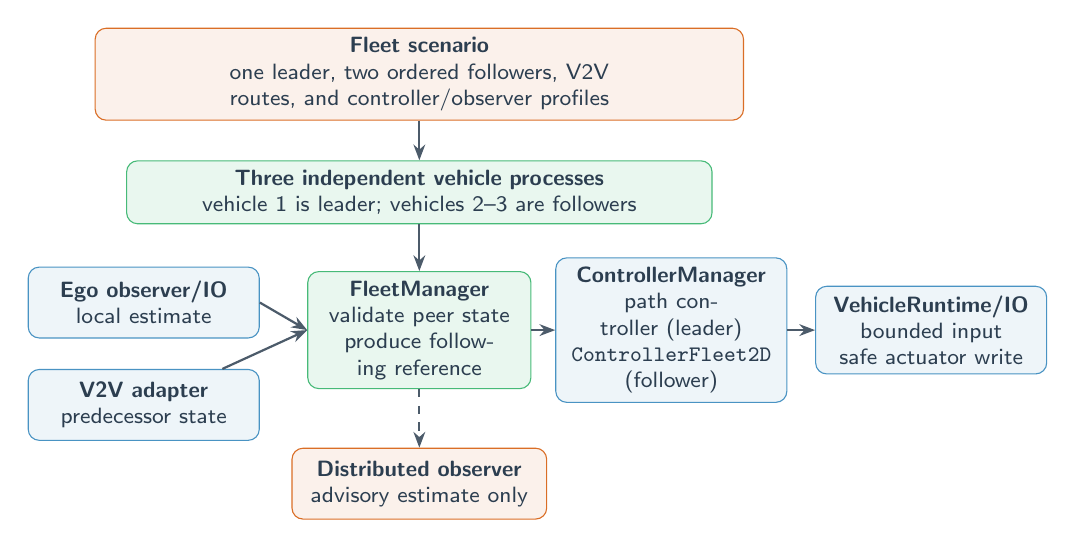
\begin{tikzpicture}[
  font=\sffamily\footnotesize,
  config/.style={rectangle,rounded corners=4pt,draw=accent!85,fill=accent!8,text=darkgray,align=center,text width=8.0cm,minimum height=.7cm},
  core/.style={rectangle,rounded corners=4pt,draw=success!85,fill=success!10,text=darkgray,align=center,text width=7.2cm,minimum height=.74cm},
  module/.style={rectangle,rounded corners=4pt,draw=primary!85,fill=primary!8,text=darkgray,align=center,text width=2.7cm,minimum height=.9cm},
  fleet/.style={module,draw=success!85,fill=success!10,text width=2.6cm},
  observer/.style={module,draw=accent!85,fill=accent!8,text width=3cm},
  arrow/.style={-{Stealth[length=2mm]},draw=darkgray!85,line width=.8pt},
  dashedarrow/.style={arrow,dashed}
]
\node[config] (scenario) at (0,3.7) {\textbf{Fleet scenario}\\one leader, two ordered followers, V2V routes, and controller/observer profiles};
\node[core] (process) at (0,2.2) {\textbf{Three independent vehicle processes}\\vehicle~1 is leader; vehicles~2--3 are followers};
\node[module] (ego) at (-3.5,0.8) {\textbf{Ego observer/IO}\\local estimate};
\node[fleet] (fleet) at (0,.45) {\textbf{FleetManager}\\validate peer state\\produce following reference};
\node[module] (control) at (3.2,.45) {\textbf{ControllerManager}\\path controller (leader)\\\texttt{ControllerFleet2D} (follower)};
\node[module] (runtime) at (6.5,.45) {\textbf{VehicleRuntime/IO}\\bounded input\\safe actuator write};
\node[module] (v2v) at (-3.5,-0.5) {\textbf{V2V adapter}\\predecessor state};
\node[observer] (distributed) at (0,-1.5) {\textbf{Distributed observer}\\advisory estimate only};
\draw[arrow] (scenario) -- (process);
\draw[arrow] (process) -- (fleet);
\draw[arrow] (ego.east) -- (fleet.west);
\draw[arrow] (fleet.east) -- (control.west);
\draw[arrow] (control.east) -- (runtime.west);
\draw[arrow] (v2v) -- (fleet.west);
\draw[dashedarrow] (fleet.south) -- (distributed.north);
\end{tikzpicture}
\caption{Fleet composition and runtime flow. Each vehicle process repeats the same local structure; only typed V2V predecessor-state messages cross between processes. The distributed observer remains advisory and has no actuation path.}
\label{fig:fleet-architecture}
\end{figure*}

The formation becomes active only after each follower receives a current predecessor state. A missing, stale, invalid, or out-of-order message triggers the fleet safety response; 

The local runtime remains the only component that writes actuator commands.

\subsection{Follower controller and distributed observer}
The leader uses the normal {\it pathplanner} and {\it ego controller}. Each follower uses the \textbf{ControllerFleet}: it places a virtual target behind its direct predecessor and tracks that target. With follower speed $v_i$, predecessor pose $(x_p,y_p,\theta_p)$, and follower pose $(x_i,y_i,\theta_i)$, first compute the target distance $d^\star$ and speed $v^\star$:
\[d^\star=d_0+h\max(0,v_i)\]
\[v^\star=\operatorname{sat}_{[0,v_{\max}]}\!\left(v_p+k_d(\lVert p_p-p_i\rVert-d^\star)\right)\]
then compute the virtual target pose $(x_v,y_v,\psi_v)$ and steering command $\delta$ by:
\[p_v=p_p-d^\star[\cos\theta_p,\sin\theta_p]^\top\]
\[\psi_v=\operatorname{atan2}(y_v-y_i,x_v-x_i)\]
\[a =  \operatorname{sat}_{[-a_{\max},a_{\max}]}\!\left(k_v * (v^\star - v_i)\right)\]
\[\delta=\operatorname{sat}_{[-\delta_{\max},\delta_{\max}]}\!\left(k_\psi\operatorname{wrap}(\psi_v-\theta_i)\right)\]
Here $d_0=5$~m and $h=0.5$~s. The speed error produces bounded throttle, and $\delta$ is the bounded steering command.

\texttt{DistributedObserverLuenberger} is an advisory prediction--correction prototype. It combines the local estimate with validated peer snapshots to form a collective estimate for diagnostics. It does not provide a controller reference or actuator command, so this report does not claim a validated distributed-observer control result. Observer theory and validation remain the next-report task.

\subsection{Fleet trajectory and spacing result}
The recorded run executed 800 cycles per vehicle (about 40~s at 50~ms per cycle). Figure~\ref{fig:fleet-summary} shows the CARLA trajectories, physical predecessor spacing, vehicle speeds, and steering commands. After the initial formation transient, both predecessor spacings converge close to their speed-dependent targets while the three vehicles continue through the curved route.

\begin{figure}[H]
\centering
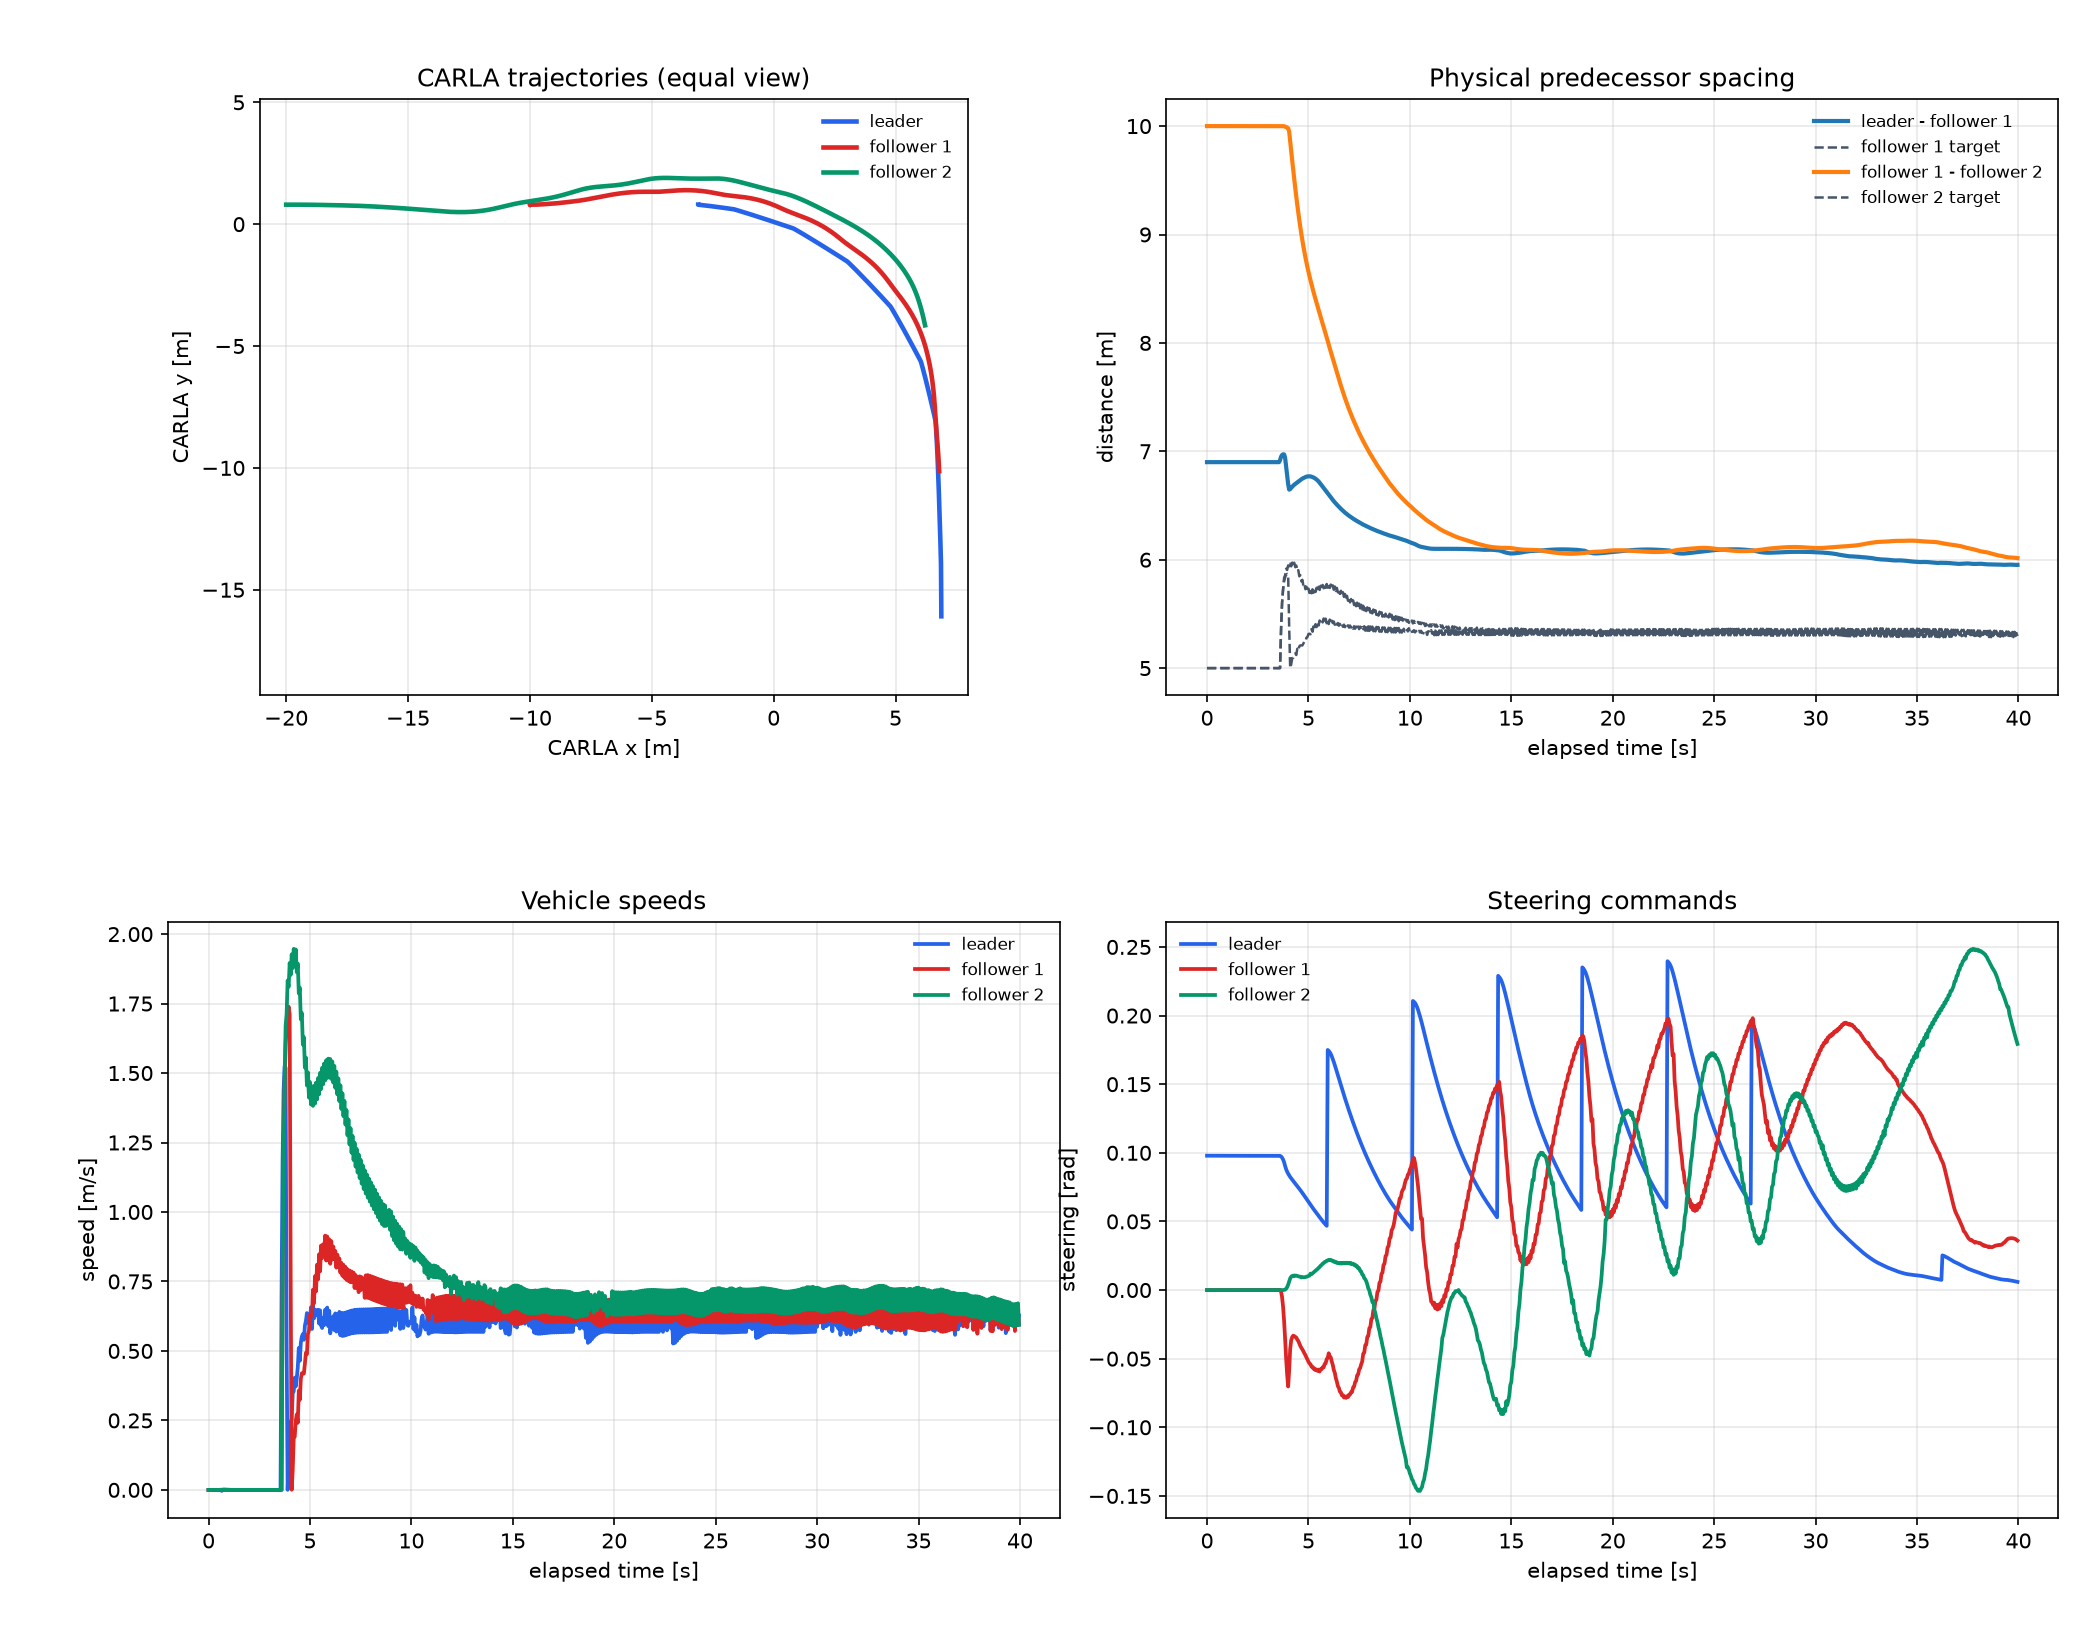
\includegraphics[width=\columnwidth]{../../test/artifacts/carla_fleet_control/fleet_carla_summary.png}
\caption{Three-vehicle CARLA fleet result: trajectories, predecessor spacing, speed, and steering command.}
\label{fig:fleet-summary}
\end{figure}

Figure~\ref{fig:fleet-diagnostics} shows that the formation moves from building to active at the start of the run and remains active. The V2V sequence-gap counter remains zero in this local CARLA run, and both followers keep advisory distributed estimates for the other two vehicles.

\begin{figure}[H]
\centering
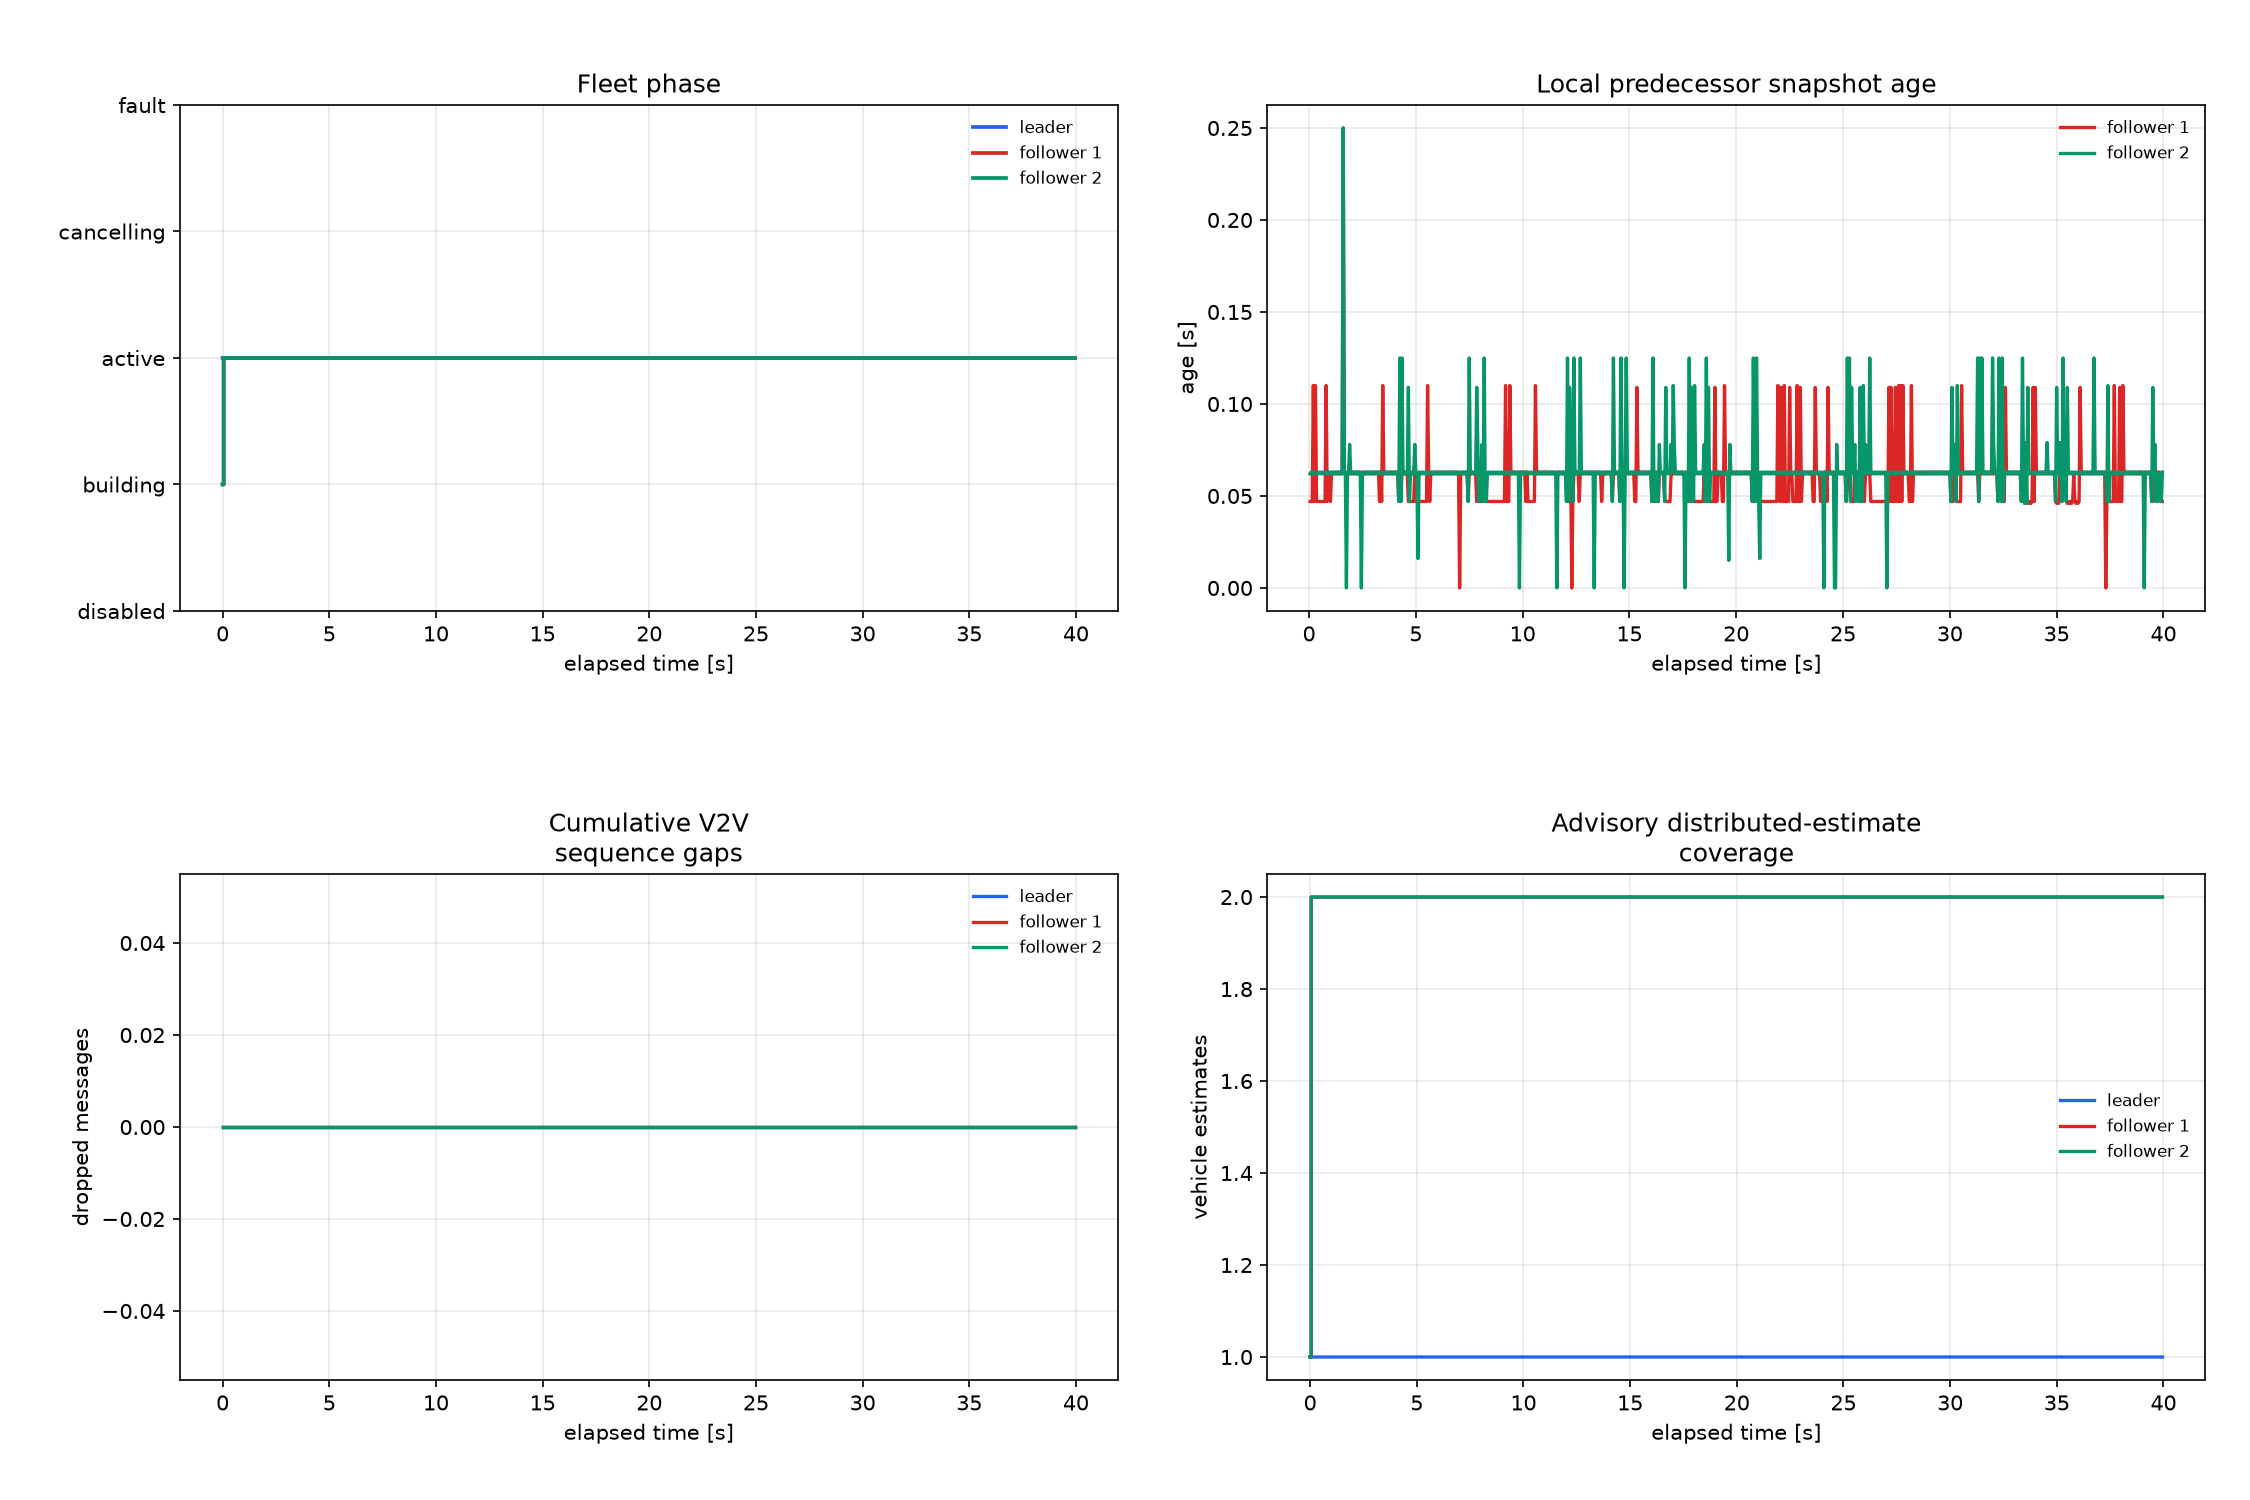
\includegraphics[width=\columnwidth]{../../test/artifacts/carla_fleet_control/fleet_carla_summary_diagnostics.png}
\caption{Fleet diagnostics: lifecycle phase, predecessor-message age, V2V sequence gaps, and distributed-estimate coverage.}
\label{fig:fleet-diagnostics}
\end{figure}

\begin{table}[H]
\centering\scriptsize
\setlength{\tabcolsep}{2pt}
\begin{tabular}{@{}p{2.05cm}p{5.3cm}@{}}
\toprule
\textbf{Check} & \textbf{Recorded result}\\
\midrule
Fleet composition & Three processes: one leader and two ordered followers.\\
Runtime duration & 800 cycles per vehicle, corresponding to approximately 40~s.\\
Follower control & Both followers enter the active phase and use the fleet 2D controller with non-zero throttle and steering.\\
Safety spacing & The integration check requires a physical gap of at least 4~m and bounds steady-state error relative to the speed-dependent spacing reference.\\
V2V health & Predecessor freshness and sequence-gap counters are recorded; this local run shows no sequence gaps.\\
Distributed observer & The leader keeps one local estimate and each follower maintains advisory coverage for all three fleet vehicles.\\
\bottomrule
\end{tabular}
\caption{Recorded CARLA fleet-control evidence.}
\label{tab:fleet-results}
\end{table}

\section{Ground-station integration}

\subsection{Design and safety boundary}
The ground station is an external operator process, not part of the vehicle runtime.

It exchanges bounded, versioned MessagePack frames over TCP. The vehicle-side bridge runs its socket work in a background thread, but that thread never calls the runtime directly. Instead, the runtime facade drains queued typed commands at its normal step boundary, returns acknowledgements, and publishes monitoring snapshots.

\begin{figure}[H]
\centering
\resizebox{\columnwidth}{!}{%
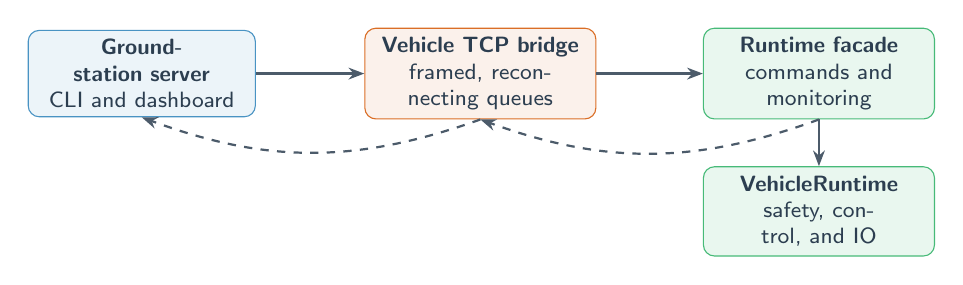
\begin{tikzpicture}[
  font=\sffamily\footnotesize,
  operator/.style={rectangle,rounded corners=4pt,draw=primary!85,fill=primary!9,text=darkgray,align=center,text width=2.65cm,minimum height=.9cm},
  transport/.style={rectangle,rounded corners=4pt,draw=accent!85,fill=accent!8,text=darkgray,align=center,text width=2.7cm,minimum height=.9cm},
  runtime/.style={rectangle,rounded corners=4pt,draw=success!85,fill=success!10,text=darkgray,align=center,text width=2.7cm,minimum height=.95cm},
  arrow/.style={-{Stealth[length=2mm]},draw=darkgray!85,line width=.8pt},
  dashedarrow/.style={arrow,dashed}
]
\node[operator] (server) at (-4.3,0) {\textbf{Ground-station server}\\CLI and dashboard};
\node[transport] (bridge) at (0,0) {\textbf{Vehicle TCP bridge}\\framed, reconnecting queues};
\node[runtime] (facade) at (4.3,0) {\textbf{Runtime facade}\\commands and monitoring};
\node[runtime] (vehicle) at (4.3,-1.75) {\textbf{VehicleRuntime}\\safety, control, and IO};
\draw[arrow] (server) -- (bridge);
\draw[dashedarrow] (bridge.south) to[bend right=-20] (server.south);
\draw[arrow] (bridge) -- (facade);
\draw[dashedarrow] (facade.south) to[bend right=-20] (bridge.south);
\draw[arrow] (facade) -- (vehicle);
\end{tikzpicture}}
\caption{Ground-station communication boundary. Transport queues data but does not bypass vehicle safety or direct IO ownership.}
\label{fig:ground-station}
\end{figure}

\subsection{Difference from the original ground station}
The structure of the ground station has changed significantly.

The original ground station was a GUI-centred application with one TCP listener per vehicle. The current ground station is a protocol-centred operator service: all vehicles connect to one configured listener and identify themselves with a versioned registration frame.

This makes the server independent of a fixed vehicle count and allows it to represent connection, stale, and reconnection states explicitly.

\begin{table}[H]
\centering\tiny
\setlength{\tabcolsep}{2pt}
\begin{tabular}{@{}p{1.5cm}p{3cm}p{3.5cm}@{}}
\toprule
\textbf{Aspect} & \textbf{Original ground station} & \textbf{Current ground station}\\
\midrule
Network identity & One listener for each vehicle; identity inferred from the port. & One listener; a vehicle sends a versioned \texttt{REGISTER} frame containing its ID.\\
Scheme & GUI, connection handling, and vehicle-specific workflows were closely coupled. & CLI/dashboard, server routing, TCP bridge, runtime facade, and vehicle runtime have separate responsibilities.\\
Command path & Commands were carried in application-specific messages to a vehicle connection. & Typed \texttt{VehicleCommand} values are validated at the runtime step boundary and return a correlated acknowledgement.\\
Safety & Ground-station features were integrated with the legacy vehicle application. & Transport cannot call the runtime or write actuators; \texttt{VehicleRuntime} remains the sole safety and IO owner.\\
Operator evidence & GUI-oriented status and feature views. & Uniform monitoring snapshots expose runtime/fleet phase, estimates, V2V health, peer age, stale/disconnected state, and command outcome.\\
Compatibility & Legacy port and message conventions. & Deliberately a new bounded MessagePack protocol; no per-vehicle-listener compatibility bridge is retained.\\
\bottomrule
\end{tabular}
\caption{Architectural comparison of the original and current ground stations.}
\label{tab:ground-station-comparison}
\end{table}

\subsection{Live operator view}
Figure~\ref{fig:ground-station-screen} is a live snapshot taken during the three-vehicle CARLA fleet experiment. The upper part of the screenshot shows the three vehicles in the CARLA map. The terminal ground station below it is the operator view of the same experiment.

\begin{figure*}[t]
\centering

\includegraphics[width=.96\textwidth]{fig/image.png}
\caption{Ground-station screenshot during the three-vehicle CARLA fleet run. The CARLA scene is shown above; the operator dashboard, command log, and command input are shown below.}
\label{fig:ground-station-screen}
\end{figure*}

The \textbf{Vehicle status} panel reports that all three vehicles are connected and \texttt{RUNNING}. For each vehicle, it displays the fleet phase and role (leader or follower), estimated state, current reference, estimate validity, peer age, V2V received/loss/dropped counters, update rate, and monitoring age. The \textbf{Commands and acknowledgements} panel shows the command sent to the selected vehicle and the returned \texttt{COMMAND\_ACK}; for example, the screenshot records start and velocity commands that were applied. The bottom \textbf{Command input} panel is the operator entry point for fleet-safe commands such as \texttt{start}, \texttt{stop}, \texttt{emergency-stop}, and \texttt{set-velocity}.

\subsection{Implemented capabilities}
\begin{itemize}[leftmargin=*]
    \item \textbf{Framed protocol:} a length-prefixed, versioned MessagePack protocol supports registration, monitoring, command, acknowledgement, and error frames. The decoder accepts fragmented TCP reads and rejects invalid or oversized frames.
    \item \textbf{Reliable operator connection:} the vehicle bridge registers with the server, reconnects after a listener restart, retains only the latest monitoring snapshot, and bounds command and acknowledgement queues.
    \item \textbf{Safe command path:} CLI requests are converted to typed \texttt{VehicleCommand} instances. The runtime remains responsible for applying or rejecting commands and returns the resulting state to the operator.
    \item \textbf{Monitoring dashboard:} the terminal display shows connection state, runtime state, estimate, control reference, V2V counters, fleet peer freshness, command outcome, and stale/disconnected status.
\end{itemize}

\subsection{Verification result}
The ground-station protocol, bridge, runtime facade, server, and dashboard were verified by the unit test suite. The 28 checks passed, covering frame fragmentation and validation, command conversion, command--snapshot--acknowledgement flow, duplicate ID rejection, stale and disconnected dashboard rows, listener restart/reconnection, bounded queues, and manual-input coalescing.

\begin{table}[H]
\centering\scriptsize
\setlength{\tabcolsep}{2pt}
\begin{tabular}{@{}p{2.0cm}p{5.3cm}@{}}
\toprule
\textbf{Area} & \textbf{Verified behaviour}\\
\midrule
Protocol & Incremental frame decoding, maximum frame size, and protocol-version validation.\\
Command flow & Typed commands arrive at the vehicle bridge, are drained by the facade, and return an acknowledgement.\\
Connection lifecycle & Vehicle registration, duplicate live-ID protection, stop handling, and reconnect after a server restart.\\
Dashboard & Latest monitoring data, stale sessions, disconnected sessions, fleet fault reason, and missing-peer display.\\
Queue policy & Bounded normal command queue and newest-value coalescing for high-rate manual input.\\
\bottomrule
\end{tabular}
\caption{Ground-station verification coverage.}
\label{tab:ground-station-results}
\end{table}

\section{Conclusion and next step}
The refactored platform now has a three-vehicle CARLA fleet result and an operator-facing ground-station boundary. The fleet artifacts show formation activation, predecessor spacing, follower control, and V2V health; the ground station provides controlled commands and readable monitoring without giving the transport layer direct control authority.

The next weekly report will add the theoretical observer result and the SDCS small-map path-following result. Those results will build on this verified fleet, CARLA, V2V, and ground-station foundation.

\end{document}
